\chapter{Moonflow}

\begin{enumerate}
    \item \formation{\tidus}{\kimahri}{\auron}
    \item Walk north, \sd\ on \kimahri\ Scene.
    \item Before Belgemine, go right into alcove and \pickup{Lv. 1 Key Spheres x3}
    \item Walk north, \sd, walk left, \sd, walk left past 2 screens, \sd.
\end{enumerate}
\begin{spheregrid}
    \begin{itemize}
        \wakkaf (7 S.Lvl) (if you don't have enough, skip this Grid entirely)
        \begin{itemize}
            \item Move $\rightarrow x4 (\downarrow)$Silence Attack
            \item +2 Strength
        \end{itemize}
        \ifthenelse{\equal{\colstyle}{multi}}{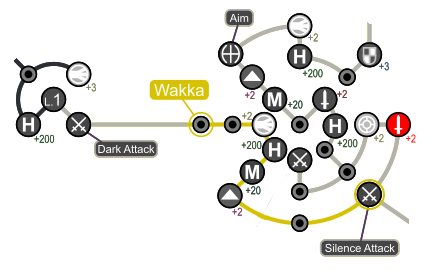
\includegraphics[width=.9\columnwidth]{graphics/Wakka_Grid}}{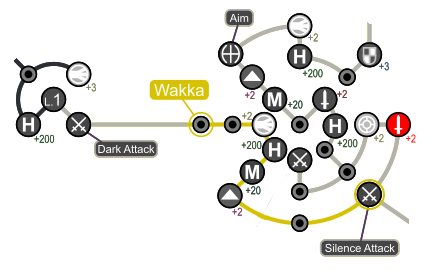
\includegraphics[width=.45\columnwidth]{graphics/Wakka_Grid}}
    \end{itemize}
\end{spheregrid}
\begin{equip}
    \begin{itemize}
        \item \textit{If you don't have Thunder Ball:}
        \begin{itemize}
            \wakkaf Official Ball
        \end{itemize}
        \item \textit{If you had Lighting Steel:}
        \begin{itemize}
            \tidusf Stunning Steel
        \end{itemize}
    \end{itemize}
\end{equip}
\begin{enumerate}[resume]
    \item Potion/Cure \tidus\ if he got injured. Walk right and use the \nth{2} option to ride ze shoopuf, \sd.
\end{enumerate}
\winvfill\lossvfill
\begin{battle}[4000]{Extractor}
    \begin{itemize}
        \tidusf Haste self
        \wakkaf Attack
        \tidusf Attack Extractor until you apply Slow
        \item \textit{If Extractor is not Slowed when it Rises:}
        \begin{itemize}
            \wakkaf \od\ Thunder Reels.
        \end{itemize}
        \tidusf Haste Wakka
        \textit{If Lightning Steel:}
        \begin{itemize}
            \tidusf Cheer x1
            \tidusf Equip Lightning Steel
        \end{itemize}
        \textit{Else:}
        \begin{itemize}
            \tidusf Cheer x4
            \tidusf Equip Brotherhood
        \end{itemize}
        \tidusf Attack
    \end{itemize}
\end{battle}
\begin{enumerate}[resume]
    \item \sd, walk left to next screen, walk left and talk to \rikku, \sd
    \item Walk up to the forced encounter
\end{enumerate}
\begin{battle}{Rikku Tutorial}
    \begin{itemize}
        \item Mash through the tutorial
        \rikkuf Steal from the Treasure Chest
        \item \textit{If you have less than 34 Power Spheres:}
        \begin{itemize}
            \rikkuf \od\ Two Ability Spheres
        \end{itemize}
        \item \textit{Else:}
        \begin{itemize}
            \rikkuf \od\ Two Potions
            \rikkuf Defend
            \item Flee
        \end{itemize}
    \end{itemize}
    +2 Power Spheres when doing the Ability Sphere Mix.
\end{battle}
\begin{spheregrid}
    \begin{itemize}
        \tidusf (4 S.Lvl)
        \begin{itemize}
            \item Move $\rightarrow\uparrow$
            \item Str+1, HP+200, Agil+2
        \end{itemize}
        \ifthenelse{\equal{\colstyle}{multi}}{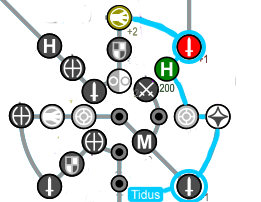
\includegraphics[width=.6\columnwidth]{graphics/Tidus_post_gui}}{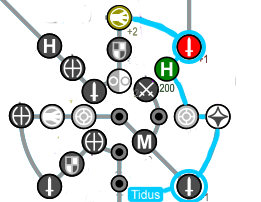
\includegraphics[width=.35\columnwidth]{graphics/Tidus_post_gui}}
    \end{itemize}
\end{spheregrid}
\begin{enumerate}[resume]
    \item Auto-Sort items
    \item Heal everyone with Potions (use them all if you can to free up the 1st Inventory Slot)
    \item If your 1st Inventory Slot is not empty Manual sort the item in that slot 1 page down
    \item \formation{\tidus}{\wakka}{\auron}
    \item Walk north to next screen.
\end{enumerate}